%!TEX TS-program = pdflatex                                          %
%!TEX encoding = UTF8                                                %
%!TEX spellcheck = en-US                                             %
%
%%%%%%%%%%%%%%%%%%%%%%%%%%%%%%%%%%%%%%%%%%%%%%%%%%%%%%%%%%%%%%%%%%%%%%
% Handout_ModelingStructuralLesions.tex
% A handout to follow during the hands-on sessions 
% 
% Authors: Timothée Proix
% 
% 
%%%%%%%%%%%%%%%%%%%%%%%%%%%%%%%%%%%%%%%%%%%%%%%%%%%%%%%%%%%%%%%%%%%%%%
% based on the tufte-latex template                                  %

\documentclass{tufte-handout}

%\geometry{showframe}% for debugging purposes -- displays the margins

\usepackage{amsmath}

% Set up the images/graphics \underline{\textbf{Analysis}}
\usepackage[pdftex]{graphicx}
\setkeys{Gin}{width=\linewidth,totalheight=\textheight,keepaspectratio}
\graphicspath{{figures/} {../../framework_tvb/tvb/interfaces/web/static/style/img/} {../../framework_tvb/tvb/interfaces/web/static/style/img/nav/}}

\title{The Virtual Brain: Hands on Session \#5}
\date{7th June 2014} 

% The following package makes prettier tables.  
\usepackage{booktabs}


% The units package provides nice, non-stacked fractions and better spacing
% for units.
\usepackage{units}
\usepackage[svgnames]{xcolor}

% The fancyvrb package lets us customize the formatting of verbatim
% environments.  We use a slightly smaller font.
\usepackage{fancyvrb}
\fvset{fontsize=\normalsize}

% Small sections of multiple columns
\usepackage{multicol}

% For adjustwidth environment
\usepackage[strict]{changepage}

% For formal definitions
\usepackage{framed}

% And some maths
\usepackage{amsmath}  % extended mathematics

% Resume a list
\usepackage{enumitem}

% Background image

\usepackage{wallpaper}

% Provides paragraphs of dummy text
\usepackage{lipsum}

% These commands are used to pretty-print LaTeX commands
\newcommand{\doccmd}[1]{\texttt{\textbackslash#1}}% command name -- adds backslash automatically
\newcommand{\docopt}[1]{\ensuremath{\langle}\textrm{\textit{#1}}\ensuremath{\rangle}}% optional command argument
\newcommand{\docarg}[1]{\textrm{\textit{#1}}}% (required) command argument
\newenvironment{docspec}{\begin{quote}\noindent}{\end{quote}}% command specification environment
\newcommand{\docenv}[1]{\textsf{#1}}% environment name
\newcommand{\docpkg}[1]{\texttt{#1}}% package name
\newcommand{\doccls}[1]{\texttt{#1}}% document class name
\newcommand{\docclsopt}[1]{\texttt{#1}}% document class option name

\newcommand\blfootnote[1]{\begingroup
         \renewcommand\thefootnote{}\footnote{\phantom{\thefootnote} #1}%
         \addtocounter{footnote}{-1}%
         \endgroup
          }

% Colours: environment derived from framed.sty: see leftbar environment definition
\definecolor{formalshade}{rgb}{0.95,0.95,1}
\definecolor{simulationshade}{rgb}{0.92, 1.0, 0.95}

% Title rule
\newcommand{\HRule}{\rule{\linewidth}{0.5mm}}

% Framed  coloured boxes

%% Blue box: for steps regarding analysis and such
\newenvironment{formal}{%
  \def\FrameCommand{%
    \hspace{1pt}%
    {\color{DarkBlue}\vrule width 2pt}%
    {\color{formalshade}\vrule width 4pt}%
    \colorbox{formalshade}%
  }%
  \MakeFramed{\advance\hsize-\width\FrameRestore}%
  \noindent\hspace{-4.55pt}% disable indenting first paragraph
  \begin{adjustwidth}{}{7pt}%
  \vspace{2pt}\vspace{2pt}%
}
{%
  \vspace{2pt}\end{adjustwidth}\endMakeFramed%
}

%% Green box: for steps regarding simulatio **only**
\newenvironment{simulation}{%
  \def\FrameCommand{%
    \hspace{1pt}%
    {\color{ForestGreen}\vrule width 2pt}%
    {\color{simulationshade}\vrule width 4pt}%
    \colorbox{simulationshade}%
  }%
  \MakeFramed{\advance\hsize-\width\FrameRestore}%
  \noindent\hspace{-4.55pt}% disable indenting first paragraph
  \begin{adjustwidth}{}{7pt}%
  \vspace{2pt}\vspace{2pt}%
}
{%
  \vspace{2pt}\end{adjustwidth}\endMakeFramed%
}

%% Orange box: for verbose descriptions
\newenvironment{blah}{%
  \def\FrameCommand{%
    \hspace{1pt}%
    {\color{DarkOrange}\vrule width 2pt}%
    {\color{PeachPuff}\vrule width 4pt}%
    \colorbox{PeachPuff}%
  }%
  \MakeFramed{\advance\hsize-\width\FrameRestore}%
  \noindent\hspace{-4.55pt}% disable indenting first paragraph
  \begin{adjustwidth}{}{7pt}%
  \vspace{2pt}\vspace{2pt}%
}
{%
  \vspace{2pt}\end{adjustwidth}\endMakeFramed%
}

%%%%%%%%%%%%%%%%%%%%%%%%%%%%%%%%%%%%%%%%%%%%%%%%%%%%%%%%%%%%%%%%%%%%%%%%%%%%%%
%                      The document starts here                              %
%%%%%%%%%%%%%%%%%%%%%%%%%%%%%%%%%%%%%%%%%%%%%%%%%%%%%%%%%%%%%%%%%%%%%%%%%%%%%%
\begin{document}
\thispagestyle{plain}
\LLCornerWallPaper{1.5}{background.png}
\begin{titlepage}
\begin{center}
% Upper part of the page. The '~' is needed because \\
% only works if a paragraph has started.

\includegraphics[width=1.5\textwidth]{./tvb_logo_transparent_square.png}~\\[0.5cm]

% Title
\begin{fullwidth}
\HRule \\[0.2cm]
\begin{center}
{ \huge \bfseries Hands-on Session \#1 \\ [0.2cm] Building Your Own Brain Network Model \\[0.1cm] }
{ \large \bfseries June 7, 2014 \\[0.2cm]}
\end{center}
\HRule \\[0.2cm]
\end{fullwidth}

\end{center}
\end{titlepage}
\newpage
\ClearWallPaper


\begin{abstract}
\noindent It is possible to use TVB to model a specific subject such as an epileptic patient. Using relevant neural
mass models, TVB allows to ask multiple questions such as the localisation of the epileptogenic zone or the validity
of different neuroimaging modalities to assess the epileptogenicity of a brain structure. Here we will present a example of
such a modelisation.
\end{abstract}

%\printclassoptions

%\begin{fullwidth} % uncomment this environment to get full texwidth paragraphs 
 
%\end{fullwidth}

\section{Objectives}\label{sec:objectives}
\newthought{The main goal} of this session is to provide a clear understanding of how we can reproduce clinically
relevant scenarios such as stimulation, modelisation of forward solution of sEEG and EEG during a seizure; modelisation of
forward solution of MEG  with interictal spikes; and, modelisation of surgery with resection of a part of the brain.

\begin{blah}
Another important step is to process data from neuroimaging modalities into TVB. We are currently developing a pipeline (github.com/timpx/scripts) that will let you easily prepare your data in a format suitable for import
into TVB. All you will need for this pipeline will be a T1 MRI and a Diffusion MRI from the subject. You can find these data
in database such as the Human Connectome project. At the end of the pipeline, you will have a connectivity, a surface and a region mapping,
i.e. you will be able to do region based and surface based simulations.
We will use the different functionalities that you have learned in the previous sessions.
\end{blah}

\subsection{Project: Session\_V\_ModellingEpilepticPatient }\label{sec:project_data}

\newthought{In this project}, all the data were already generated. We'll only go through the necessary steps 
required to reproduce the simulations listed in Table~\ref{tab:simtab}, along with the relevant outline.
You can always start over, click along and/or try to change parameters.
We will use the default subject connectivity matrix and surface.


\begin{margintable}
  \centering
  \fontfamily{ppl}\selectfont
  \begin{tabular}{l}
    \toprule
    Name \\
    \midrule
    Exploring the Epileptor model\\
    \\
    Region based simulation of an epileptic patient \\
    $\quad$\textit{Region\_TemporalLobe} \\
    $\quad$\textit{Region\_TemporalLobe\_sEEG\_EEG}  \\
    \\
    Surface based simulation of an epileptic patient \\
    $\quad$\textit{Surface\_TemporalLobe\_sEEG\_EEG}  \\
    \\
    Applying a stimulus to trigger seizures \\
    $\quad$\textit{Surface\_Stimulation}  \\ 
    \\
    MEG forward solution for interictal spikes \\
    $\quad$\textit{Surface\_InterictalSpikes\_MEG} \\
    \\
    Modeling surgical resection\\
    $\quad$\textit{Surface\_Resection} \\
    \bottomrule
  \end{tabular}
  \caption{Simulations in this project.}
  \label{tab:simtab}
\end{margintable}

% let's start a new thought -- a new section

\subsection{Exploring the Epileptor model}\label{sec:epileptor}


\newthought{Before doing} any simulations, we would like to have a look at the phase space of the Epileptor model
to understand better its dynamics. We will use the interactive tool that you have seen in Session \#4.

\begin{formal}
  \begin{enumerate}[resume]
  \item Go to \textsc{simulator} and select the $\mathbf{Epileptor}$ model
  \item Click on \underline{Set Up Region Model}.
  \item Look at the phase space (Fig. \ref{fig:phase_space}). We have here the first population (variables $y_0$ in abscissa and 
  $y_1$ in ordinate).
  The left most intersection of the nullcline defines a stable fixed point whereas the rightmost intersection 
  is the center of a limit cycle. Both states are separated by a separatrix, as you can se by drawing different trajectories
  in this phase space (left click on the figure).
  \item You can also look at other variables in the phase space, such as $y_2$/$y_0$ (slow-fast subsystem) or 
  $y_5$/$y_4$ (second population), and change parameters to see what is the effect on the nullclines.
  \end{enumerate}
\end{formal}


\begin{figure}[h]
  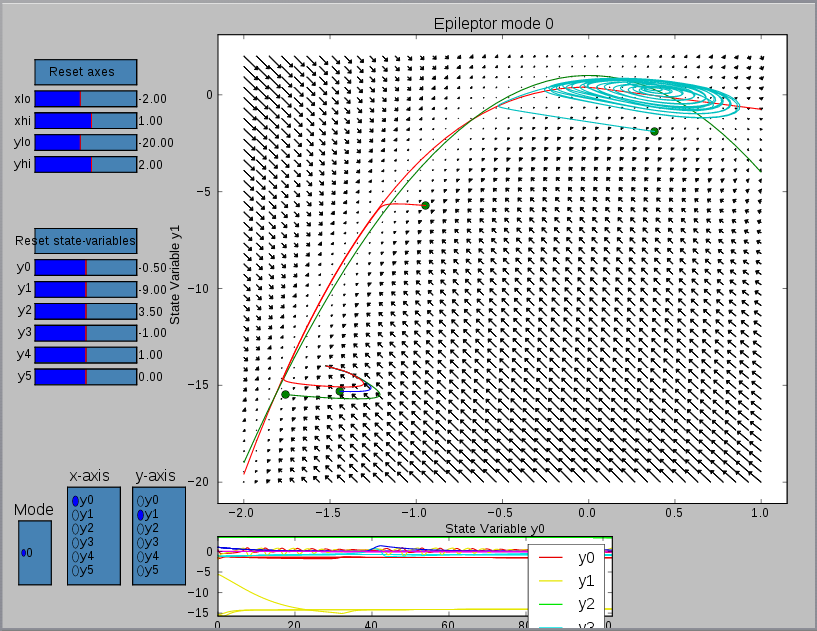
\includegraphics[width=\linewidth]{Handout_UI_ModellingAnEpilepticPatient_PhaseSpace}%
  \caption{phase space for the first population}%
  \label{fig:phase_space}%
\end{figure}
\subsection{Region based simulation of an epileptic patient}

\newthought{We are going} to model a patient with temporal lobe epilepsy (TLE). We will choose different values of
epileptogenicity ($x_0$ parameters in the Epileptor) according to the region positions, thereby introducing heterogeneities in
the model parameters (Session \#4). We set the right limbic areas 
(right hippocampus (rHC), parahippocampus (rPHC) and amygdala (rAMYG)) as epileptic zones. We also add two lesser epileptogenic regions: 
the superior temporal cortex (rTS) and the ventral temporal cortex (rTV).

\begin{simulation}
  \begin{enumerate}
  \item Stay in the same page; all nodes are selected by default, give them the value $\mathbf{-2.2}$ for the $\mathbf{x_0}$ parameter.
  \item \underline{Remove all} selected nodes, select lHC, lAMYG and lPHC, save the selection with a name
	and set the parameter $\mathbf{x_0}$ to the value $\mathbf{-1.6}$. \underline{Submit Region Parameters} values.
  \item \underline{Configure the Visualizers} and add a \underline{Brain Viewer} and a \underline{Fourier Spectrum}, 
  then \underline{Save your choices}.
  \item Choose an $\mathbf{integration\:step\:size}$ of \textbf{\unit[0.1]{ms}}, a $\mathbf{Temporal\:average\:monitor}$ with a \textbf{sampling period} of \textbf{\unit[1]{ms}} and \textbf{\unit[6000]{ms}} as a simulation length. 
  All the other parameters are
  given in the table \ref{tab:modeltab}.
 \end{enumerate}
\end{simulation}

\begin{margintable}
  \centering
  \fontfamily{ppl}\selectfont
  \begin{tabular}{ll}
    \toprule
    Model parameter & Value \\
    \midrule
             $Iext$          &   3.1  \\
             $Iext2$          &  0.45   \\
             $R$           &   0.00035        \\
             $slope$           &   0.0   \\
    \bottomrule
  \end{tabular}
  \caption{Parameters for the Epileptor model	 }
  \label{tab:modeltab}
\end{margintable}

\begin{marginfigure}
  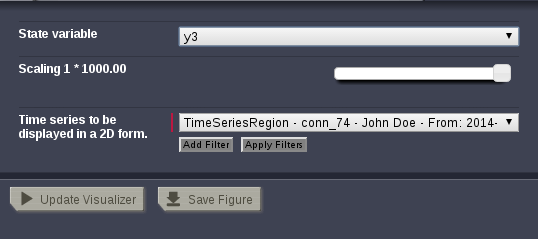
\includegraphics[width=\linewidth]{Handout_UI_ModellingAnEpilepticPatient_BrainMenu}%
  \caption{Brain menu: you can increase the scaling and change the variable to be displayed.}%
  \label{fig:brain_menu}%
\end{marginfigure}

The results are already computed for you in \textit{Region\_TemporalLobe}



\begin{simulation}
  \begin{enumerate}
  \setcounter{enumi}{4}
  \item Visualize the time series. Click on \underline{Select channels} and select all the channels. 
	You will need to increase the scaling by clicking on 
\includegraphics[width=0.08\textwidth]{butt_brain_menu}(Fig. \ref{fig:brain_menu}). Visualize 
	the $y_0$ (Fig. \ref{fig:first_pop}) then the $y_3$ state variable (Fig. \ref{fig:second_pop}) by 
	changing it in 
\includegraphics[width=0.08\textwidth]{butt_brain_menu}. You can see a succession of 3 seizures, use the mouse
	 to zoom in and out in the time series area.
  \item Visualize the results in the \underline{Brain Viewer}, you will need to increase the rendering speed 
	(timesteps per Frame) by clicking on 
\includegraphics[width=0.08\textwidth]{butt_brain_menu}.
\end{enumerate}
\end{simulation}
  
\begin{figure}[h]
  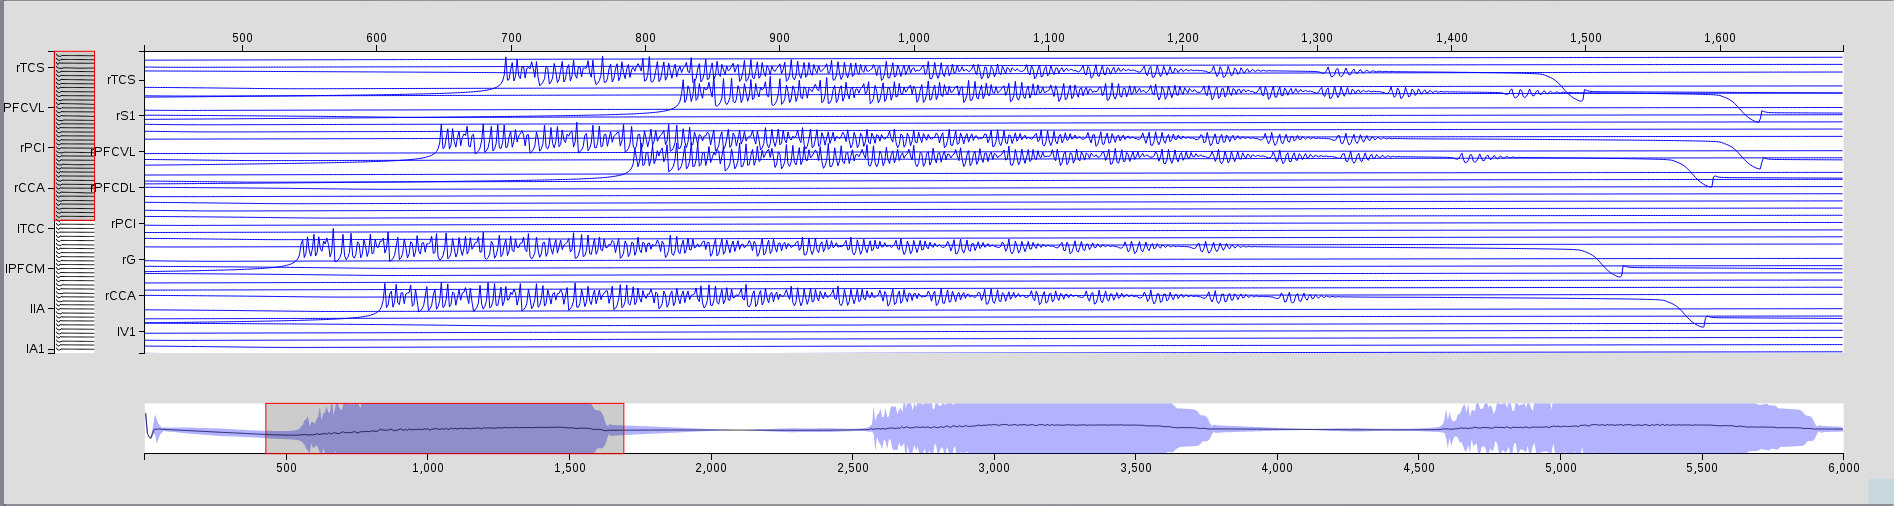
\includegraphics[width=\linewidth]{Handout_UI_ModellingAnEpilepticPatient_FirstPopulationTimeSeries}%
  \caption{Time series for the first population}%
  \label{fig:first_pop}%
\end{figure}



\begin{figure}[h]
  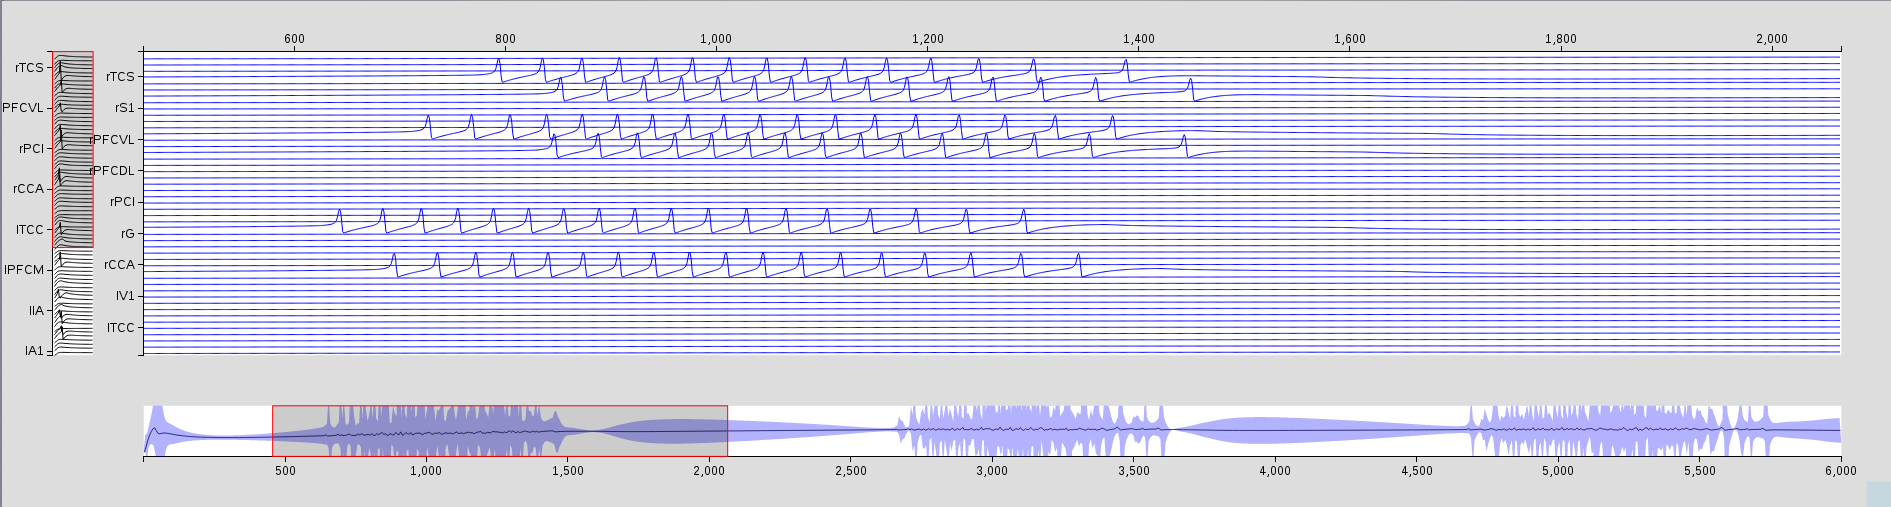
\includegraphics[width=\linewidth]{Handout_UI_ModellingAnEpilepticPatient_SecondPopulationTimeSeries}%
  \caption{Time series for the second population}%
  \label{fig:second_pop}%
\end{figure}

\begin{blah}
  \begin{enumerate}[resume]
  The length of seizures here is not realistic ($\sim$\unit[2]{s}), but you can always obtain realistic time by multiplying
  all the derivatives of the model by a small factor.
  \end{enumerate}
\end{blah}
We now are going to run this simulation again, but with intracranial electrodes (sEEG) and EEG monitors.

\begin{simulation}
  \begin{enumerate}
  \item Copy the former simulation.
  \item Add two new monitors (EEG and sEEG) with a \textbf{sampling period} of \textbf{\unit[1]{ms}} by hitting Ctrl and at the same time clicking on the monitor you want to add.
  \item For this simulation, we will not use the \underline{Brain Viewer} so reconfigure the \underline{View} tabs accordingly.
\end{enumerate}
\end{simulation}

The results are already computed for you in \textit{Region\_TemporalLobe\_sEEG\_EEG}


\begin{simulation}
  \begin{enumerate}
    \setcounter{enumi}{3}
  \item Click on \underline{Results}.
  \item Click on the EEG time series and visualize them with the 3d/2d visualizer (Fig. \ref{fig:sEEG}).
  \item Go back, click on the sEEG time series and visualize them with the 3d/2d visualizer (Fig. \ref{fig:EEG}).
\end{enumerate}
\end{simulation}



\begin{figure}[h]
  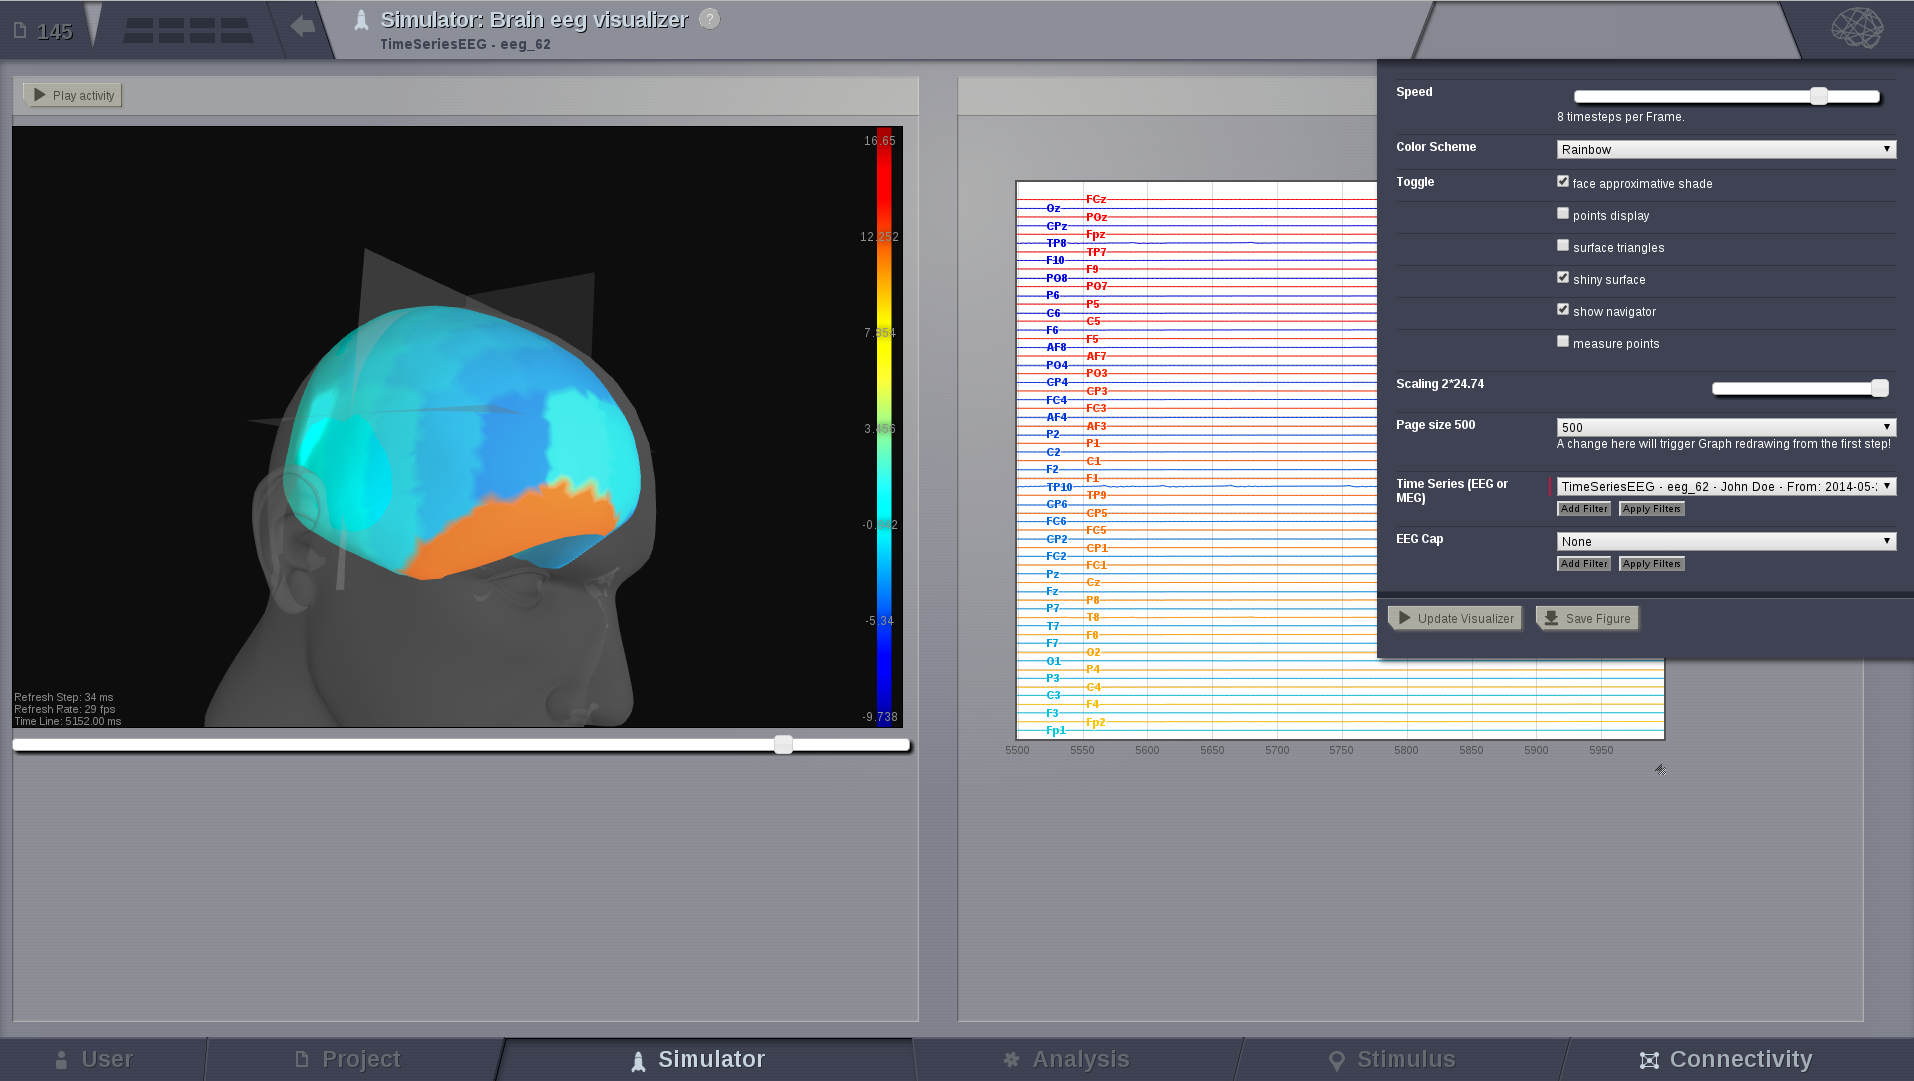
\includegraphics[width=\linewidth]{Handout_UI_ModellingAnEpilepticPatient_EEG3d2dBrainVisualizer}%
  \caption{sEEG 3d/2d visualizer}%
  \label{fig:sEEG}%
\end{figure}

\begin{figure}[h]
  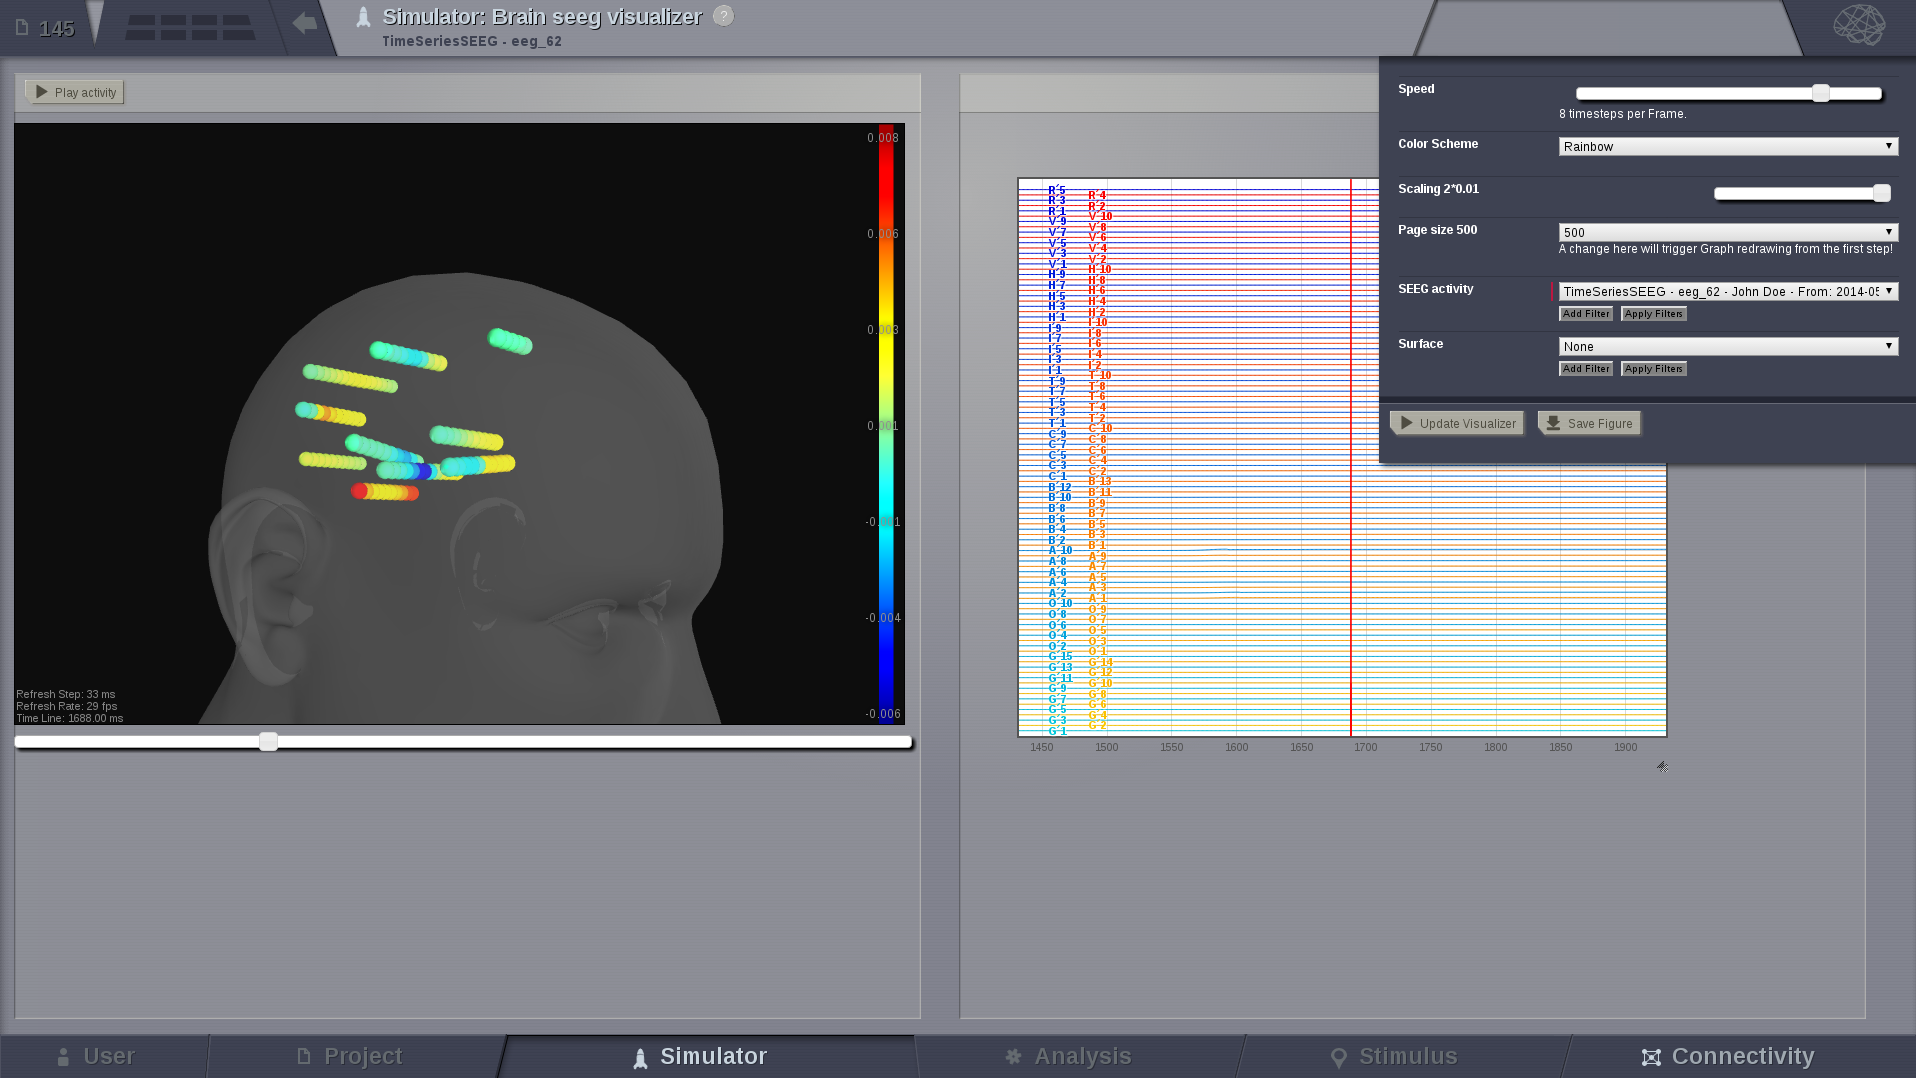
\includegraphics[width=\linewidth]{Handout_UI_ModellingAnEpilepticPatient_sEEG3d2dBrainVisualizer}%
  \caption{EEG 3d/2d visualizer}%
  \label{fig:EEG}%
\end{figure} 

\subsection{Surface based simulation of an epileptic patient}

 \newthought{To account} also for seizure propagation and not only seizure recruitment, we have to use surface based simulations.
 It also allows to have a more accurate representation of the MEG/EEG/sEEG signal.
 
  \begin{simulation}
  \begin{enumerate}
  \item Copy the former simulation.
  \item Add a \underline{Brain Viewer} visualizer.
  \item Choose the TVB's $\mathbf{default\:surface}$, the corresponding  $\mathbf{local\:connectivity}$ and a $\mathbf{Local\:coupling\:strength}$ of $\mathbf{a=0.2}$.
  \item Add a $\mathbf{Spatial\:average}$ monitor with a \textbf{sampling period} of \textbf{\unit[1]{ms}}
  \item Click on \underline{Set up surface model} (Fig. \ref{fig:set_up_surface_parameters}). Choose working parameters
  ($\mathbf{Model\:parameter\:x_0}$, $\mathbf{Equation:\:Gaussian}$, $\mathbf{amp=0.6}$, $\mathbf{sigma=10.}$, $\mathbf{offset=-2.2}$) and 
  click on \underline{Apply equation}.
  Click on a location on the brain where you want the parameter setting to apply, then click on \underline{Add focal point}.
  Then click on \underline{Submit Surface parameters}. You can see that the field of the $x_0$ parameter is updated according to the selected equation.
  \end{enumerate}
\end{simulation}

\begin{figure}[h]
  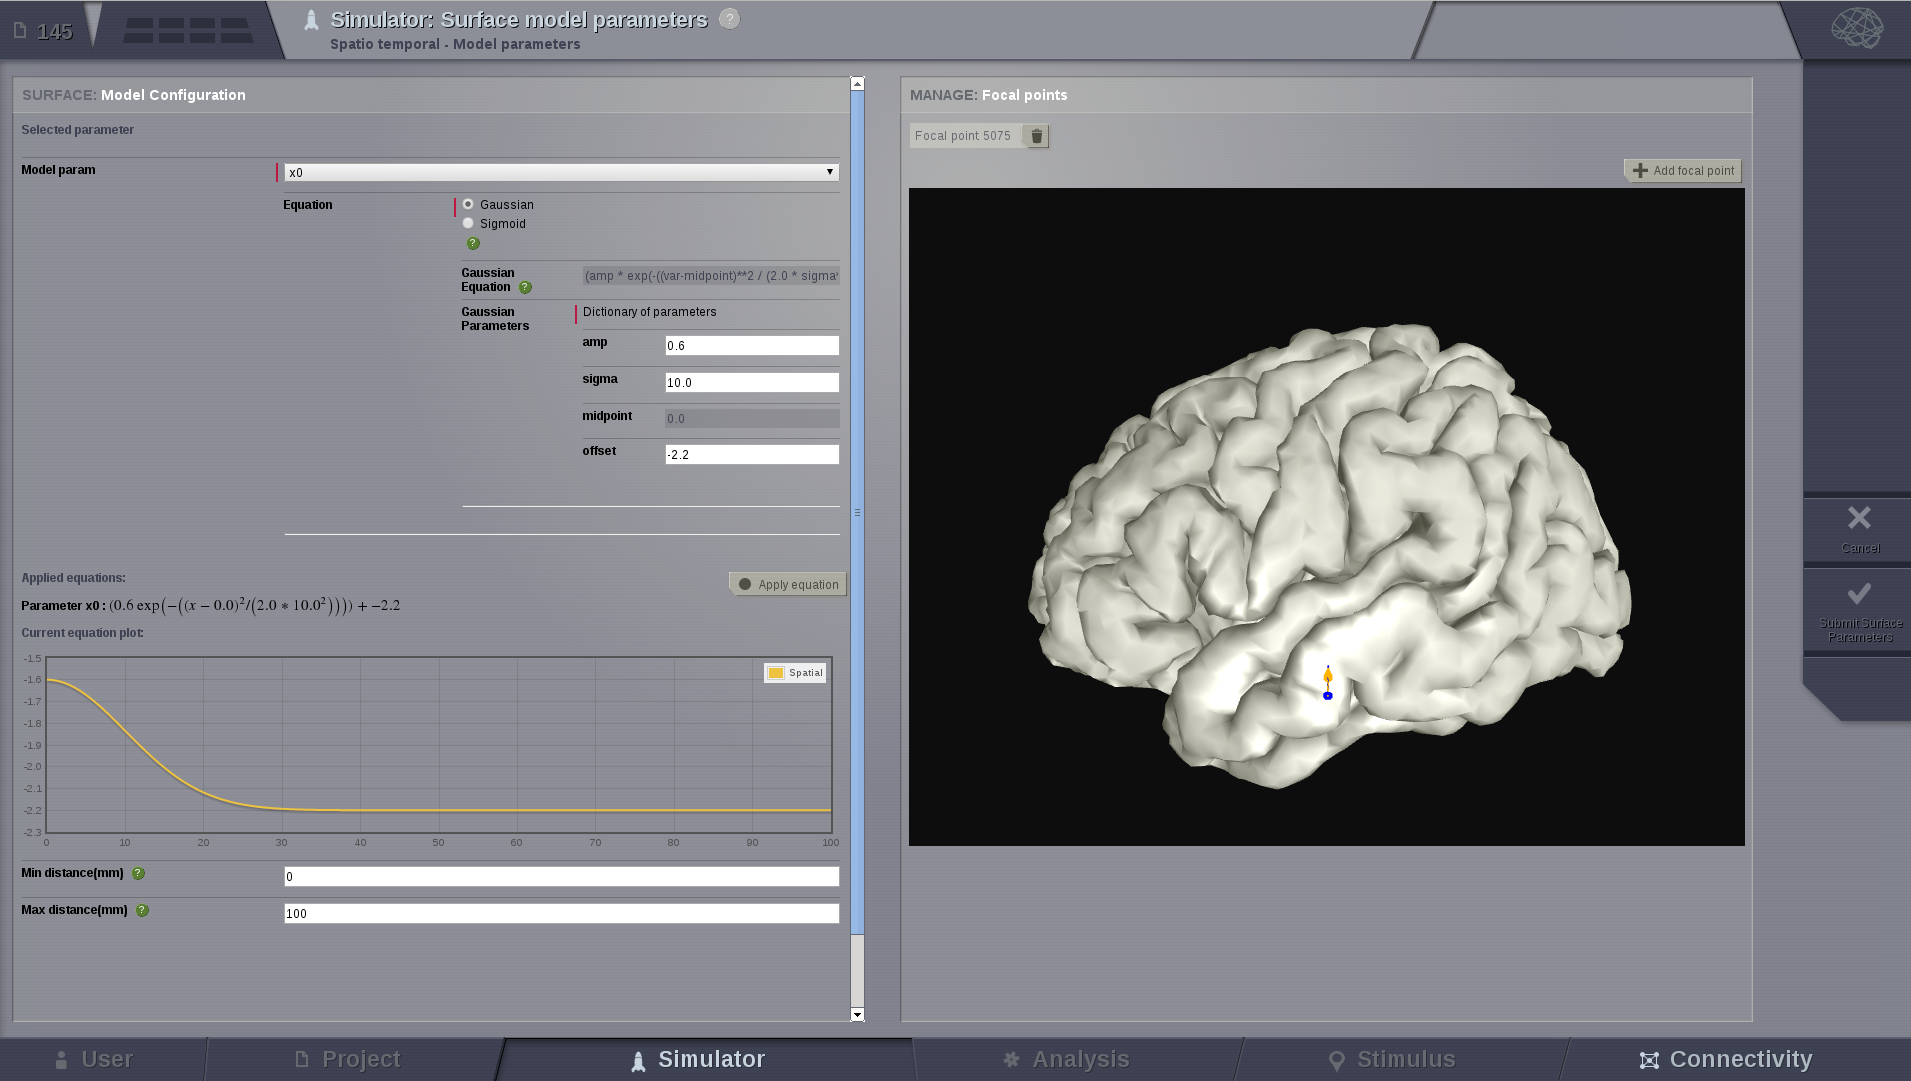
\includegraphics[width=\linewidth]{Handout_UI_ModellingAnEpilepticPatient_SetUpSurfaceParameters}%
  \caption{Set up the surface parameters}%
  \label{fig:set_up_surface_parameters}%
\end{figure}

  The results are already computed for you in \textit{Surface\_TemporalLobe\_sEEG\_EEG}
 \begin{simulation}
  \begin{enumerate}
     \setcounter{enumi}{5}
  \item Click on \underline{Results}, click on the TimeSeriesSurface an visualize them in the 
  \underline{Brain Activity Visualizer} (Fig. \ref{fig:bv_surf}). You can use the arrows of the numpad to rapidly 
  move the brain.
  \item Go back,  click on \underline{TimeSeries} and visualize them with the \underline{Time Series Visualizer}. Change the scaling, change the selected channels and zoom in to see
  the seizure (Fig. \ref{fig:ts_surf}).
  \item Go back, click on \underline{TimeSeriesSEEG} and visualize them with the 3d/2d visualizer (Fig. \ref{fig:surf_sEEG}).
  Note the difference with the former region-based simulation.
  \item Go back, click on the EEG time series and visualize them with the 3d/2d visualizer (Fig. \ref{fig:surf_EEG}).
  Note the difference with the region-based simulation.
\end{enumerate}
\end{simulation}

\begin{figure}[h]
  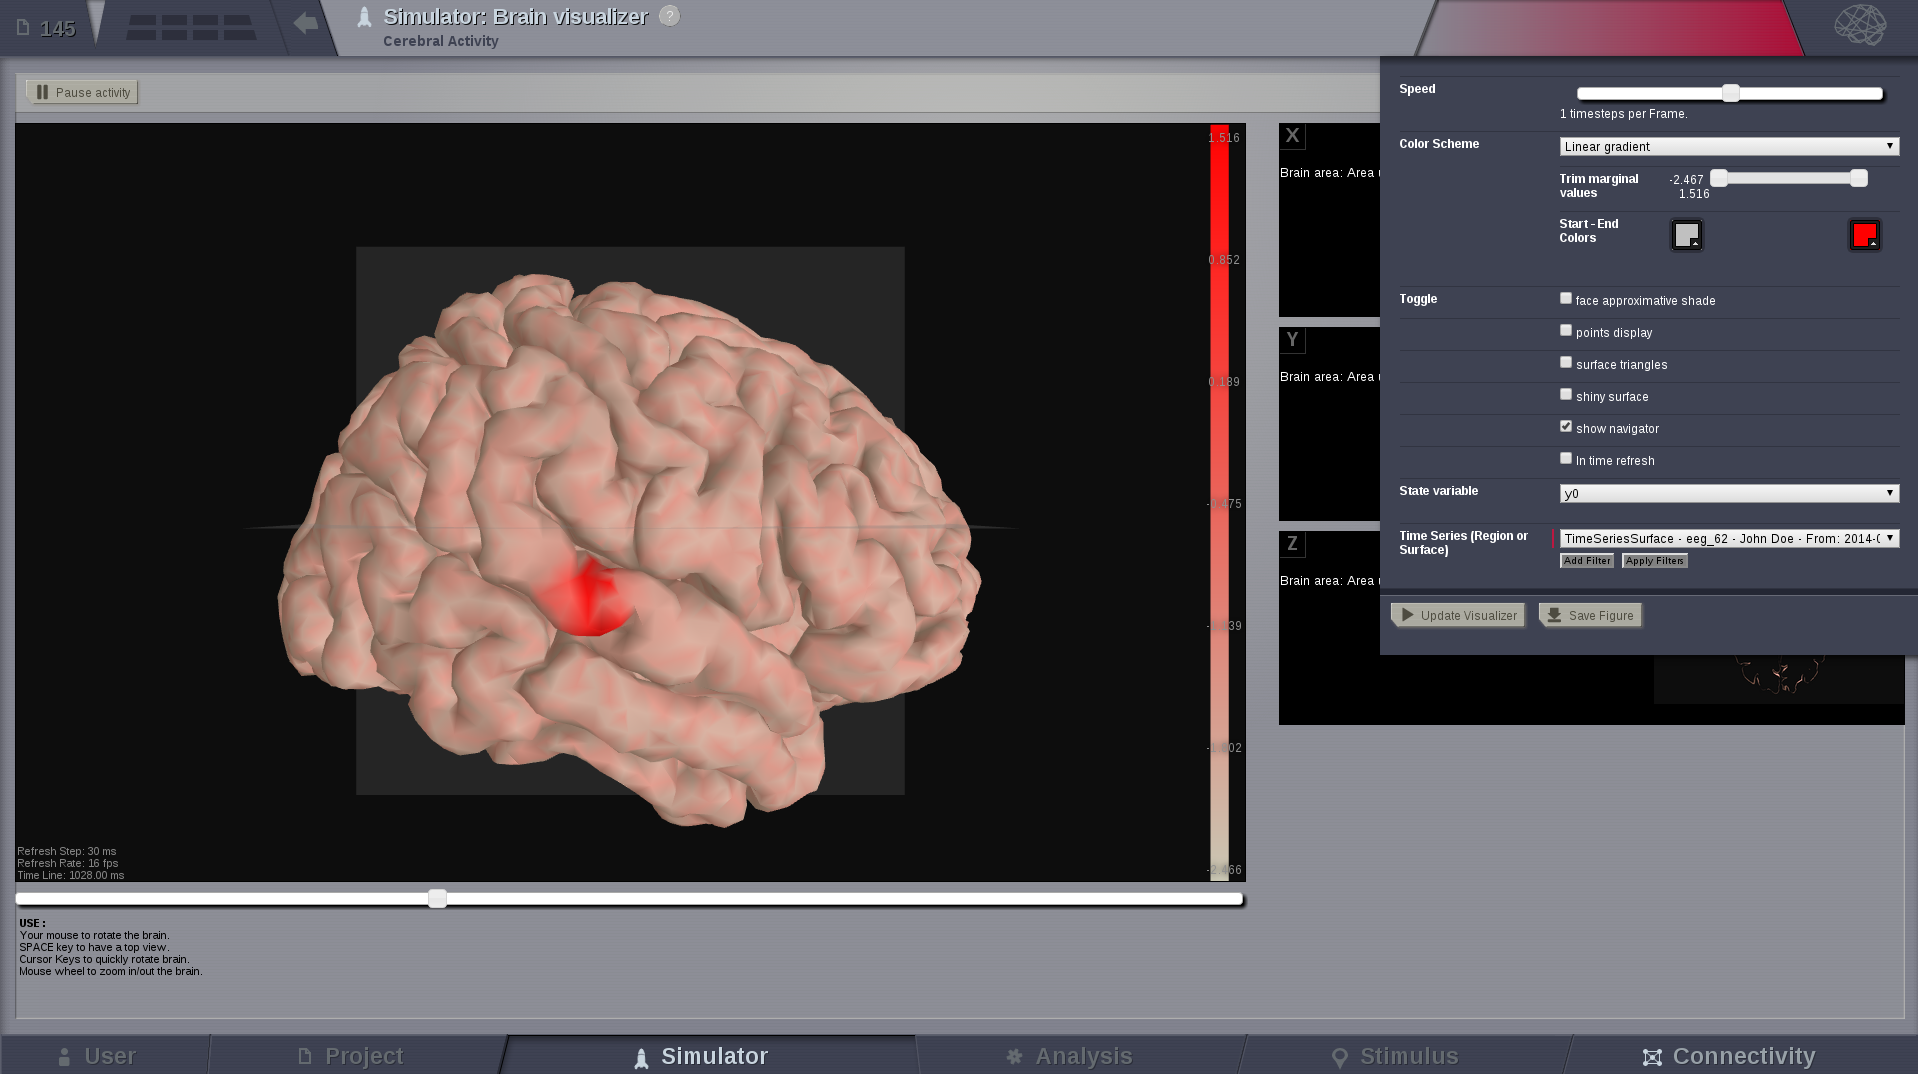
\includegraphics[width=\linewidth]{Handout_UI_ModellingAnEpilepticPatient_TemporalAverageTimeSeriesSurface}%
  \caption{Spatial averaged time series for a surface simulation}%
  \label{fig:bv_surf}%
\end{figure}

\begin{figure}[h]
  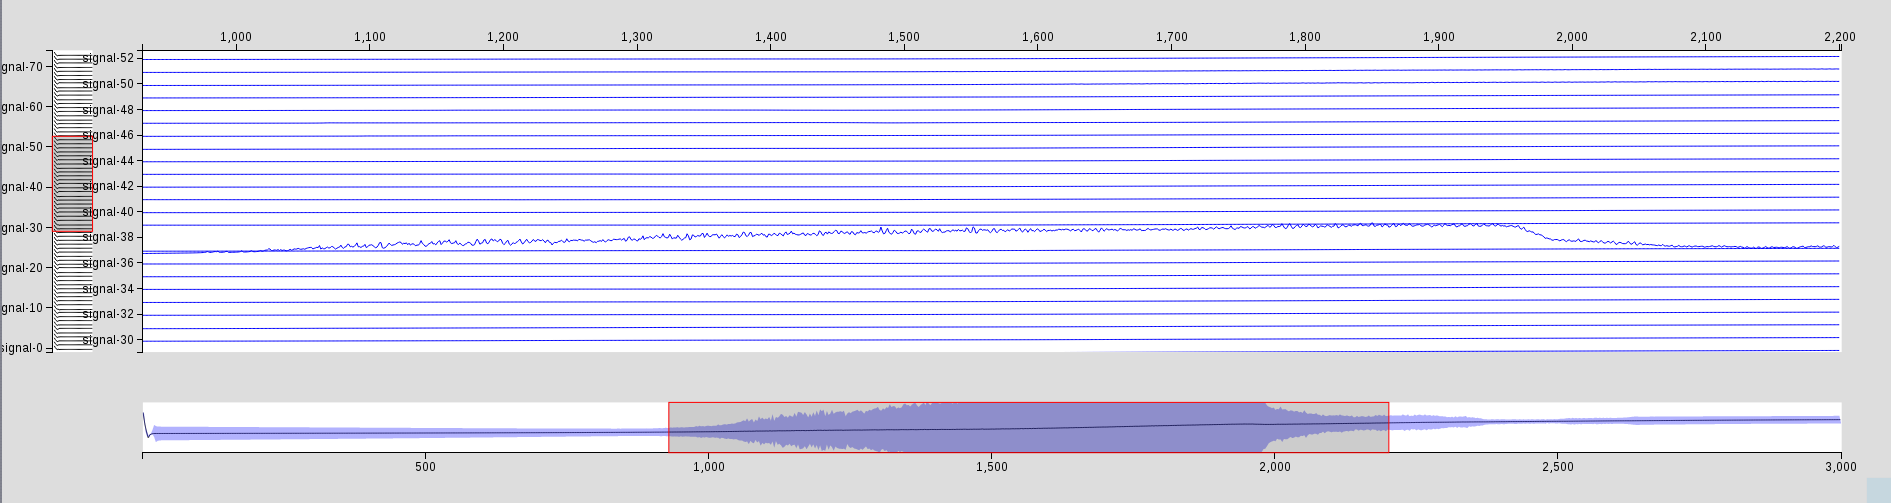
\includegraphics[width=\linewidth]{Handout_UI_ModellingAnEpilepticPatient_SpatialAverageTimeSeries}%
  \caption{Spatial averaged time series for a surface simulation}%
  \label{fig:ts_surf}%
\end{figure}

\begin{figure}[h]
  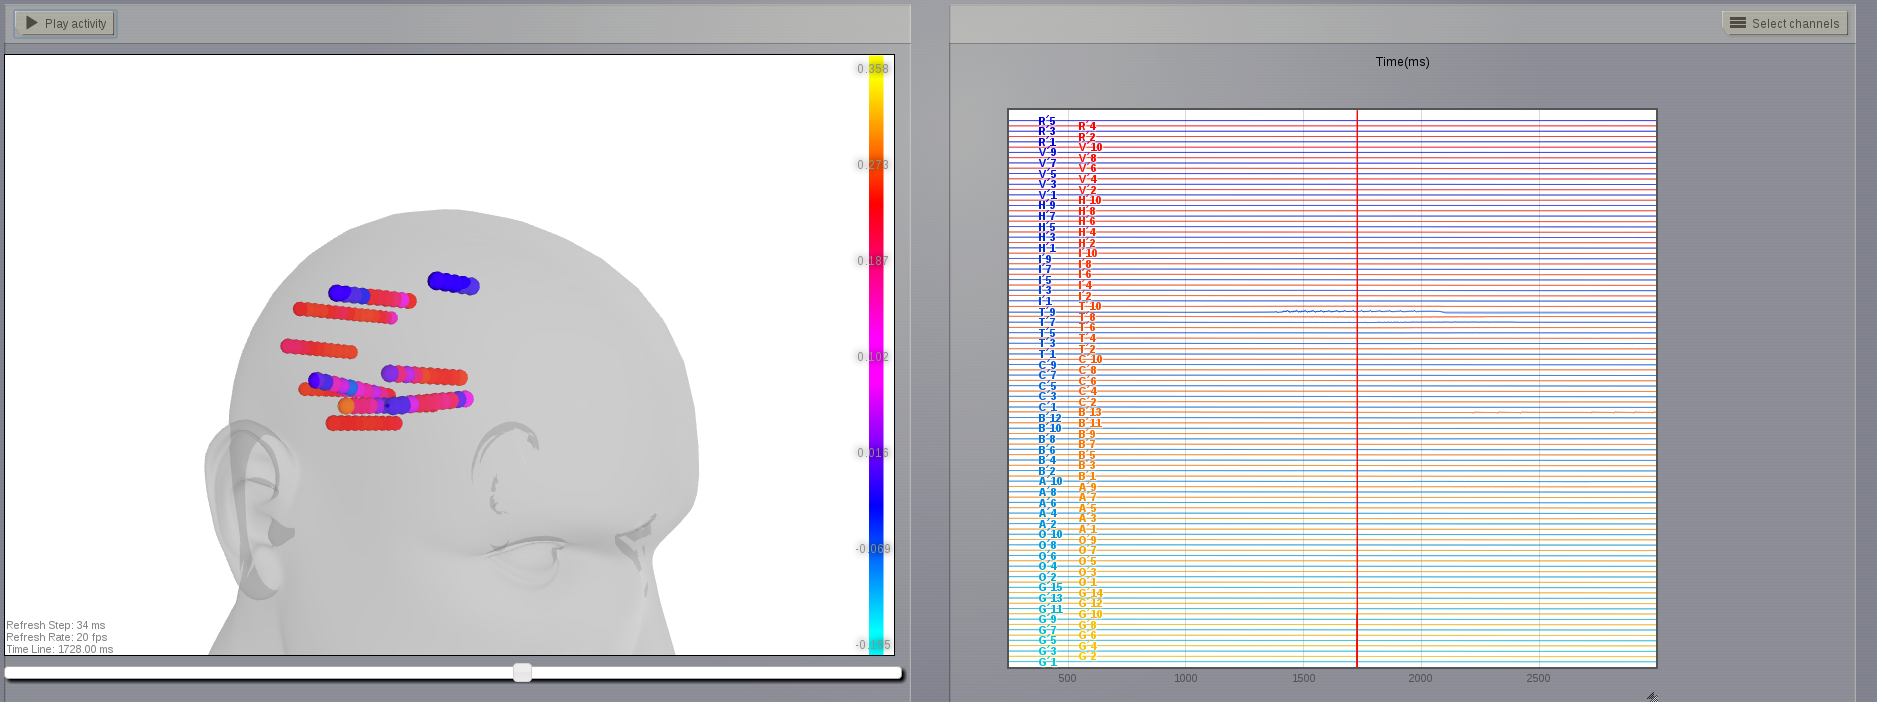
\includegraphics[width=\linewidth]{Handout_UI_ModellingAnEpilepticPatient_sEEGSurface}%
  \caption{sEEG for a surface simulation}%
  \label{fig:surf_sEEG}%
\end{figure}

\begin{figure}[h]
  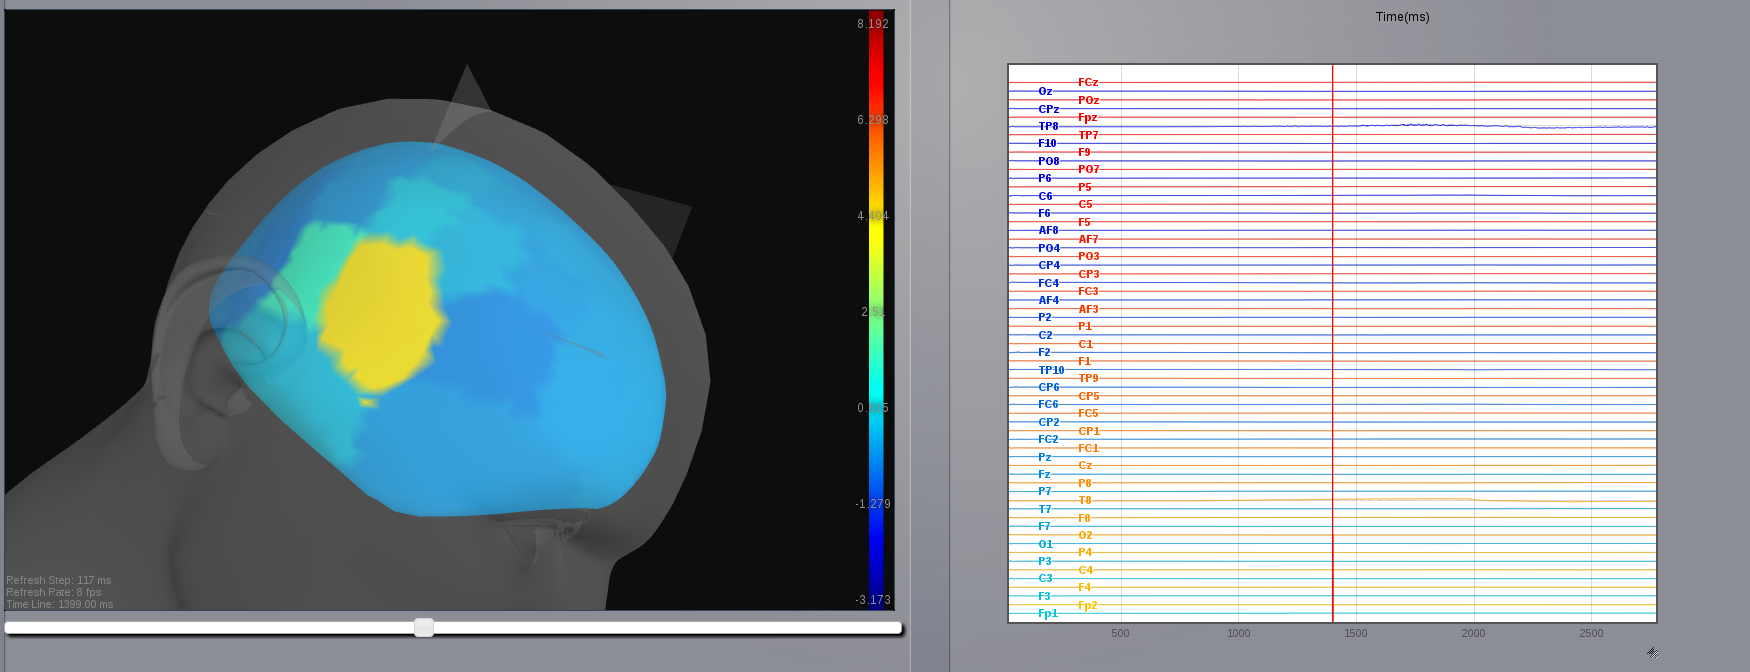
\includegraphics[width=\linewidth]{Handout_UI_ModellingAnEpilepticPatient_EEGSurface}%
  \caption{EEG for a surface simulation}%
  \label{fig:surf_EEG}%
\end{figure}

\subsection{Applying A Stimulus To Trigger Seizures}

\newthought{Now} we are going to simulate a stimulation.
We set the whole brain to non-epileptogenic but close to the threshold

\begin{margintable}
  \centering
  \fontfamily{ppl}\selectfont
  \begin{tabular}{ll}
    \toprule
    Space stimulation parameters & Value \\
    \midrule
             $amp$          &   1.0  \\
             $radius$          &  5.0   \\
             $sigma$           &   1.0        \\
             $offset$           &   0.0   \\
    \midrule
    \midrule
    Time stimulation parameters & Value \\
    \midrule
             $onset$          &   2000.0 \\
             $tau$          &  20.0   \\
             $T$           &   4000.0        \\
             $amp$           &   10.0   \\
    \bottomrule
  \end{tabular}
  \caption{Space and time parameters for the stimulus}
  \label{tab:stimtab}
\end{margintable}

  \begin{formal}
  \begin{enumerate}
  \item Go to \textsc{stimulus} $\rightarrow$ \textsc{Surface Stimulus}
  \item Give a name to the new stimulus
  \item Choose a \underline{Sigmoid} stimulation in space with the parameters given in Table \ref{tab:stimtab}
  \item Choose a \underline{PulseTrain} stimulation in time with parameters given in table \ref{tab:stimtab} (Fig. \ref{fig:stim_st})
  \item Click on \underline{Edit Focal Points and View}
  \item Choose a focal point (Fig. \ref{fig:stim_foc})
  \item \underline{Save the new stimulus on surface}
  \end{enumerate}
\end{formal}


\begin{figure}[h]
  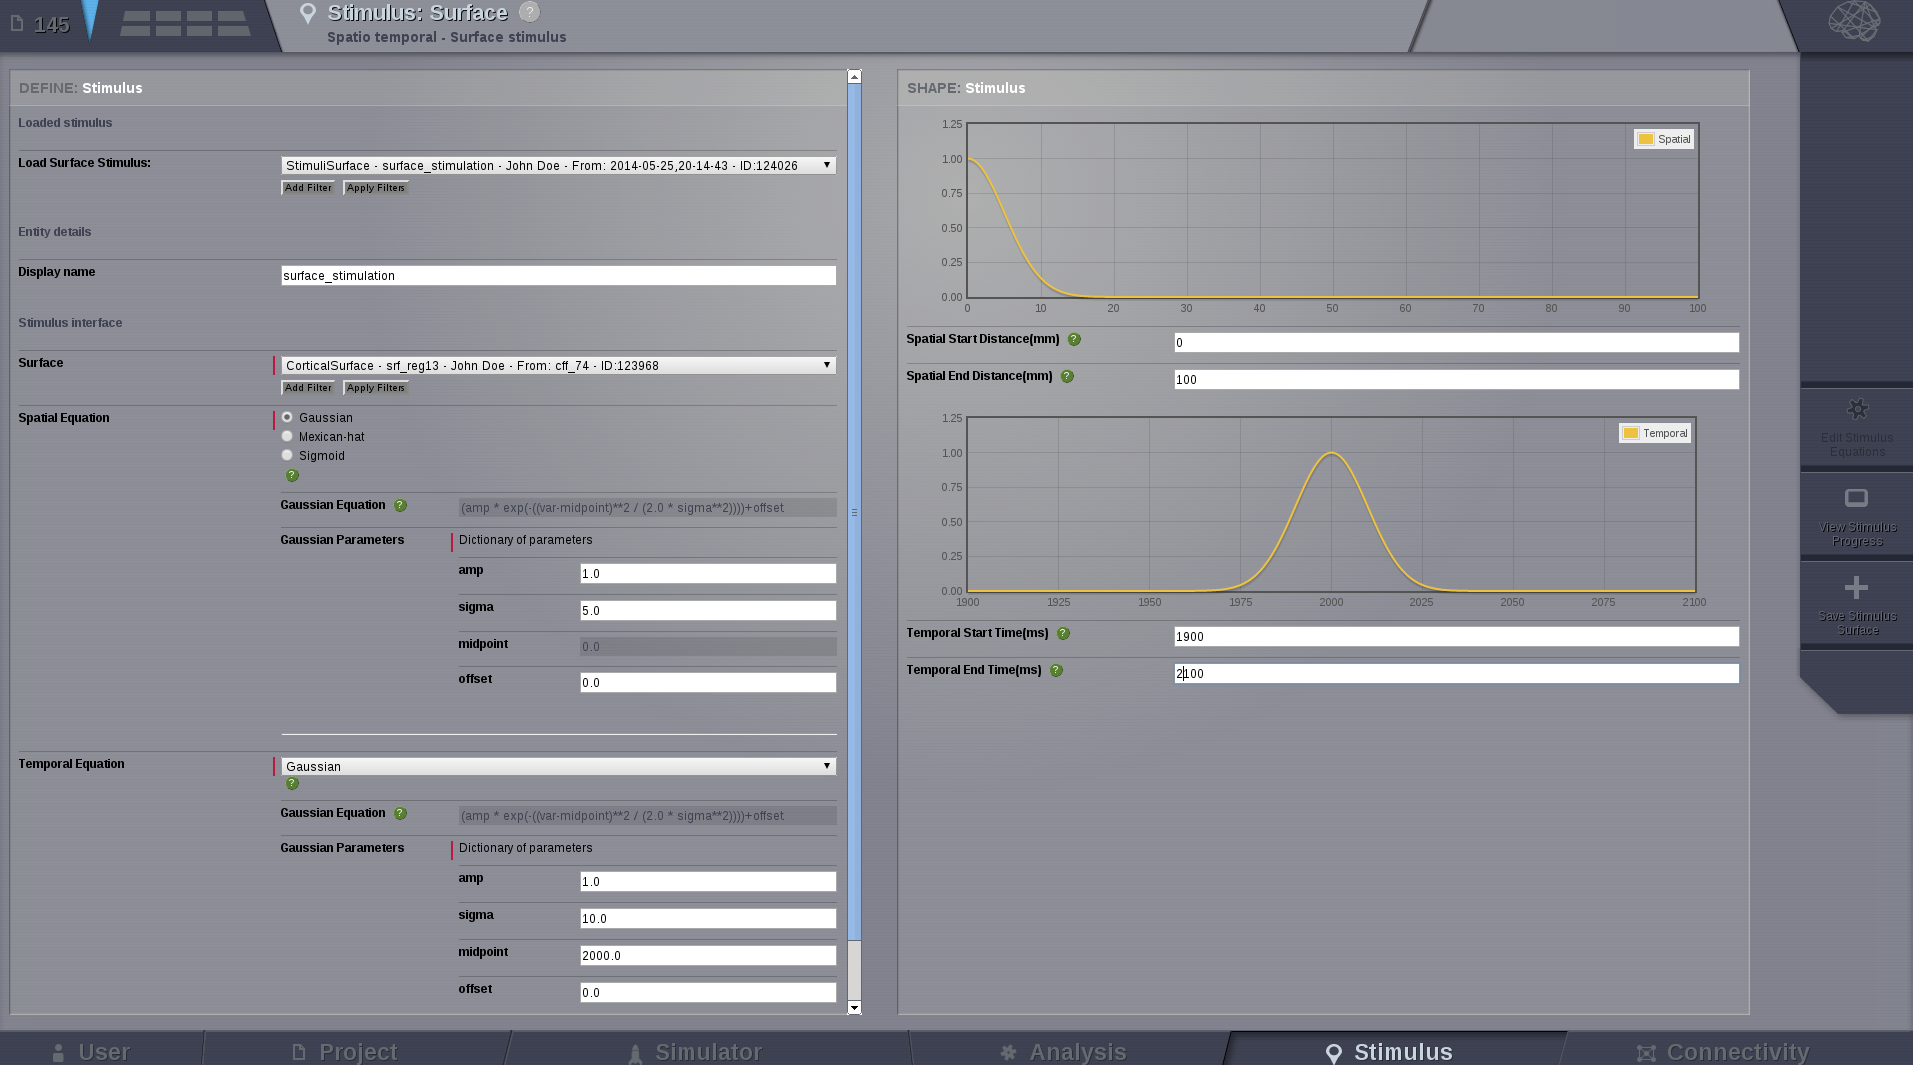
\includegraphics[width=\linewidth]{Handout_UI_ModellingAnEpilepticPatient_StimulationSpatioTemporalPattern}%
  \caption{Spatio temporal pattern of the stimulus}%
  \label{fig:stim_st}%
\end{figure}

\begin{figure}[h]
  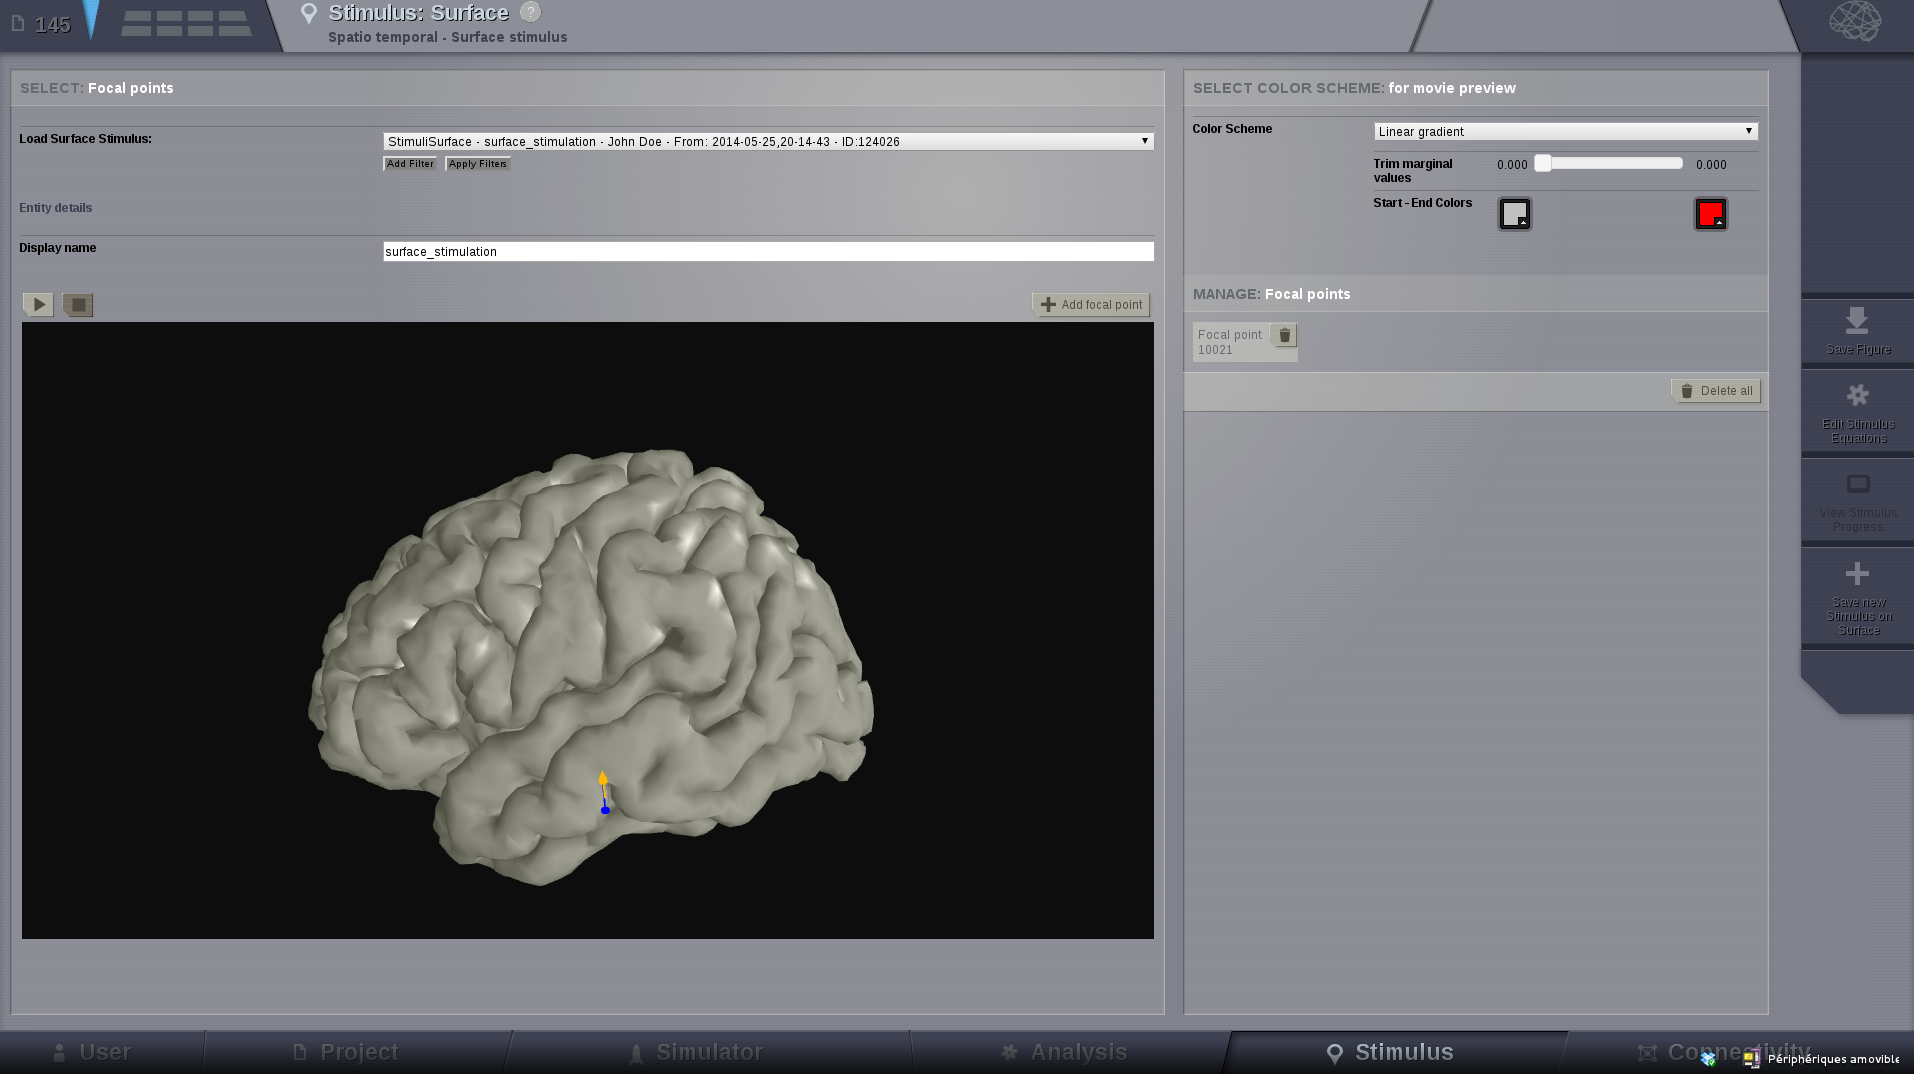
\includegraphics[width=\linewidth]{Handout_UI_ModellingAnEpilepticPatient_StimulationFocalPoint}%
  \caption{Focal point for a surface stimulation}%
  \label{fig:stim_foc}%
\end{figure}

The stimulus was already set for you under the name \textit{Surface\_SquareStimulus}

  \begin{simulation}
  \begin{enumerate}
  \setcounter{enumi}{7}
  \item Go to \textsc{simulator} and copy the former simulation.
  \item Choose the \textit{Surface\_SquareStimulus} stimulus.
  \item Set the parameter $\mathbf{x_0}$ to $\mathbf{-2.1}$
  \item Choose only a \textbf{Spatial average} monitor.
  \item Set the $\mathbf{Simulation\:Length}$ to \textbf{\unit[4000]{ms}}.
 
\end{enumerate}
\end{simulation}


You can see the result of this simulation in \textit{surface stimulation}

\begin{marginfigure}
  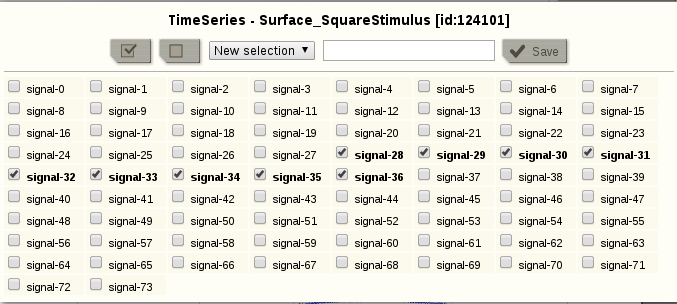
\includegraphics[width=\linewidth]{Handout_UI_ModellingAnEpilepticPatient_ChooseChannelsStimulation}%
  \caption{Channel selection menu: you can choose the channels of interest. }%
  \label{fig:choose_channels}%
\end{marginfigure}


  \begin{simulation}
  \begin{enumerate}
  \setcounter{enumi}{12}
  \item Click on \underline{Results}, click on the TimeSeries and visualize the Surface Average Time Series with 
  the \underline{Animated Time Series} visualizer.
  \item \underline{Select channel} \#67 to \#73 (Fig. \ref{fig:choose_channels}). Increase the page size in 
\includegraphics[width=0.08\textwidth]{butt_brain_menu} to include time \textbf{\unit[2000]{ms}}
  (Fig. \ref{fig:bm_stim}) and better see the effect of the stimulation (Fig. \ref{fig:stim_ts}).
 
\end{enumerate}
\end{simulation}


\begin{figure}[h]
  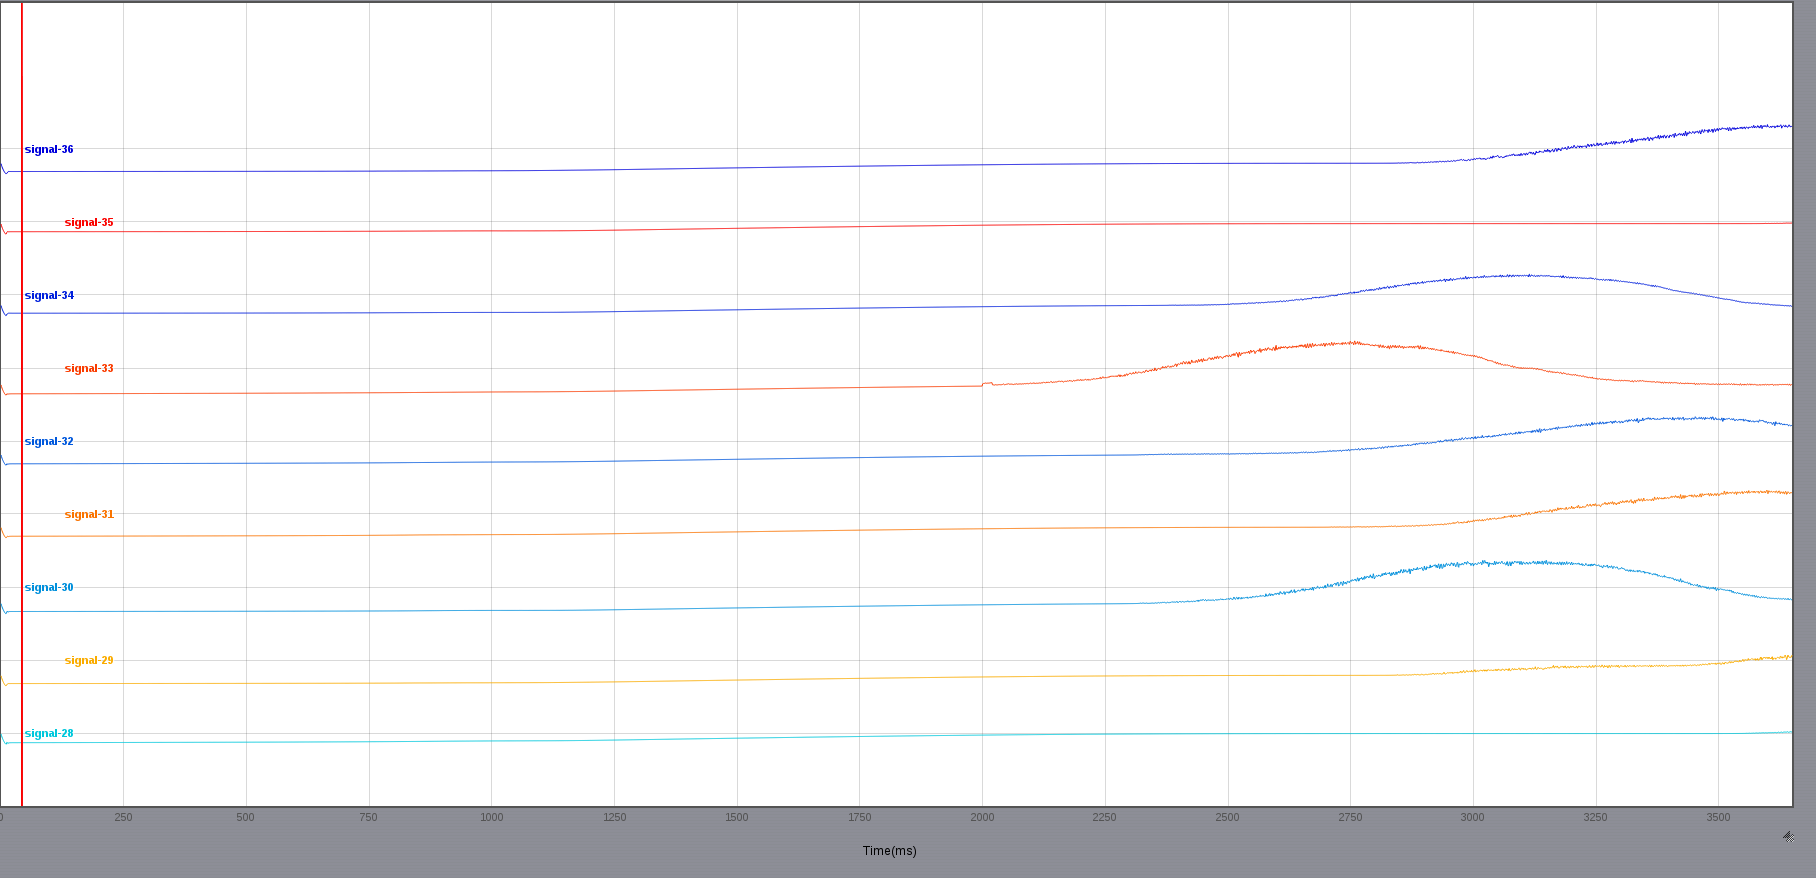
\includegraphics[width=\linewidth]{Handout_UI_ModellingAnEpilepticPatient_StimulationTimeSeries}%
  \caption{Time Series for a stimulation}%
  \label{fig:stim_ts}%
\end{figure}

\begin{marginfigure}
  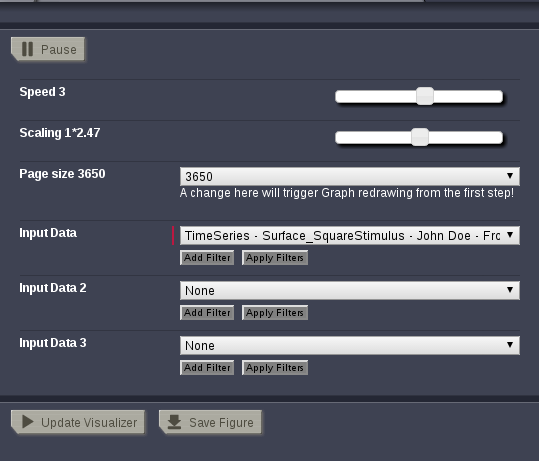
\includegraphics[width=\linewidth]{Handout_UI_ModellingAnEpilepticPatient_BrainMenuStimulation}%
  \caption{Brain menu: Increase the scaling to see the time \unit{2000}[ms].}%
  \label{fig:bm_stim}%
\end{marginfigure}

\subsection{MEG forward solution for interictal spikes}

\newthought{MEG is rarely} recorded during a seizure and usually we have only access to interictal recordings.
Therefore it is interesting to simulate interictal spikes in order to test forward and inverse model in MEG.
We are going to set the parameter $\mathbf{x_0}$ in such a way that the Epileptor model will not trigger seizures, but only interictal spikes, 
i.e. the model will be set close to the threshold between ictal and interictal states. 
We will also add noise to trigger the interictal spikes.

  \begin{simulation}
  \begin{enumerate}
  \item Copy the former simulation.
  \item Set the \textbf{Spatiotemporal Stimulus} back to the \textbf{None} value.
  \item As we did earlier, go to \underline{Set Up region Model} and set the $\mathbf{x_0}$ parameter to $\mathbf{-3.0}$ for all 
  nodes except for the selection \textit{right\_amy\_hip\_parahip} for which you set the value $\mathbf{-2.1}$ and for the selection
  \textit{right\_orbital\_temporal} for which you set the value $\mathbf{-2.8}$.
  \item Choose a \textbf{HeunStochastic} integration scheme with a \textbf{integration step-size} of $\mathbf{0.05}$. We choose
  a smaller integration time step than previously to be sure that  the integration scheme stays stable even in presence of noise.
  We will put noise in the two variables of the second population which are responsible for triggering interictal spikes:
  set $\mathbf{D}$ to $\mathbf{[0., 0., 0., 0.002, 0.002, 0.]}$.
  \item Choose the \textbf{MEG} monitor with a sampling period of \textbf{\unit[1]{ms}}
\end{enumerate}
\end{simulation}

The results are given in \textit{Surface\_InterictalSpikes\_MEG}.

  \begin{simulation}
  \begin{enumerate}
  \item Go to \underline{Results}, select the \underline{MEG Time series} and visualize them wit the \underline{Time Serie Visualizer}.
  Choose \underline{channels} $\#15$, $\#73$, $\#84$ and $\#150$ and increase the \underline{scaling}, you should see interictal spikes on this MEG simulation 
  (Fig. \ref{fig:ts_meg}).
\end{enumerate}
\end{simulation}

\begin{figure}[h]
  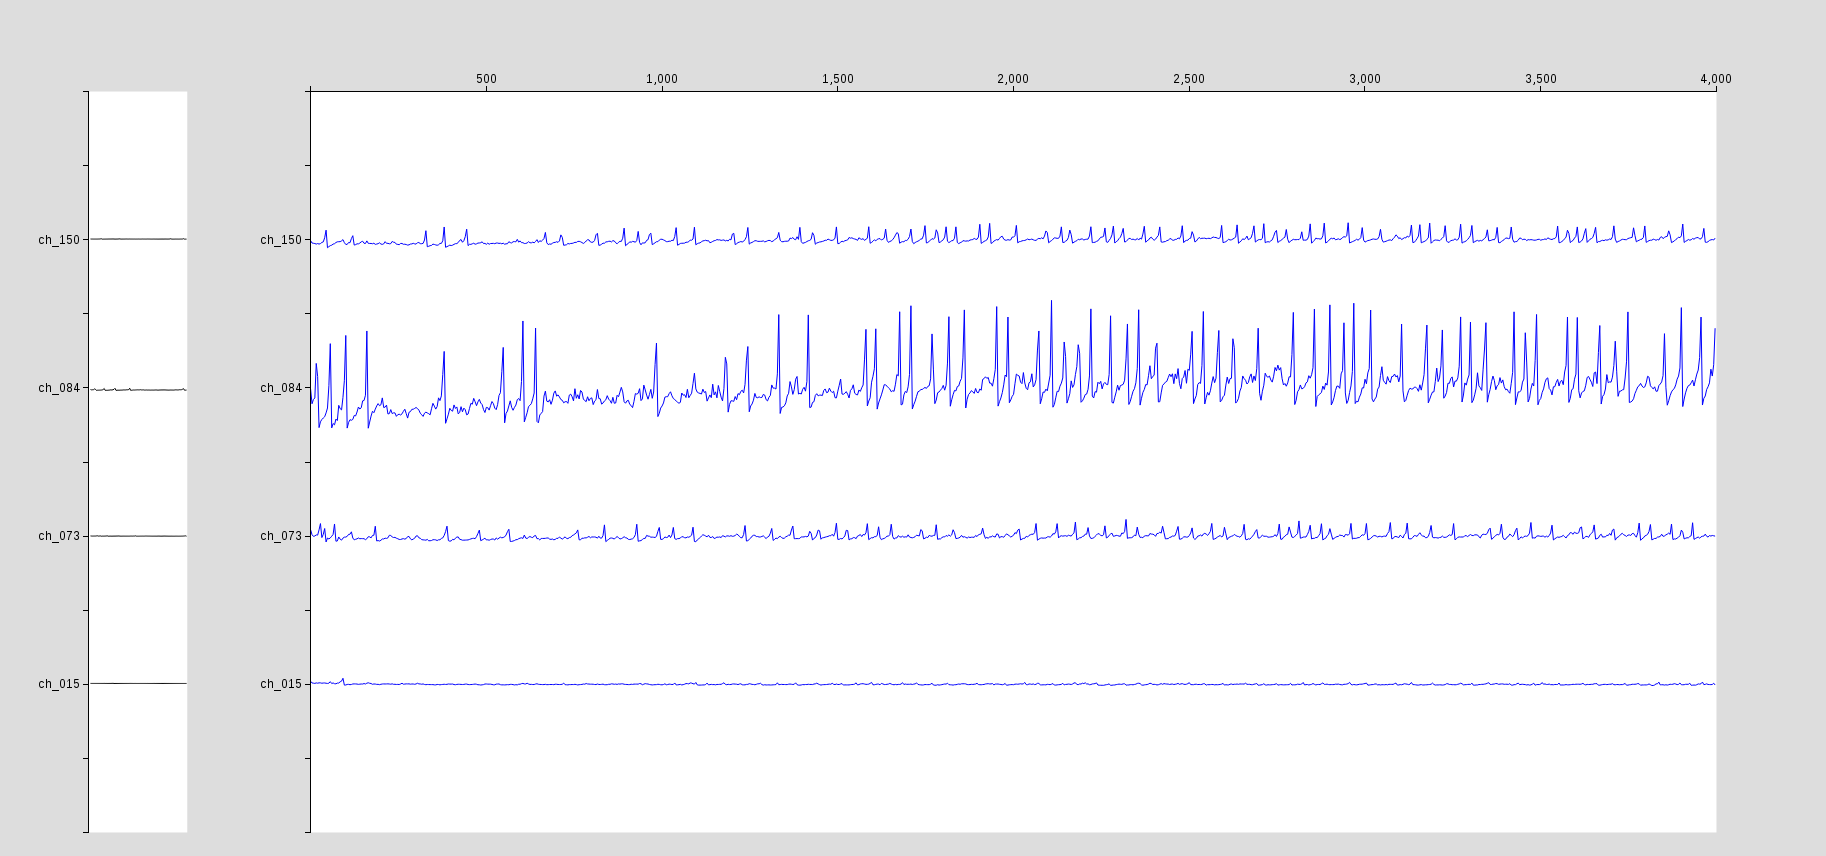
\includegraphics[width=\linewidth]{Handout_UI_ModellingAnEpilepticPatient_MEGTimeSeries}%
  \caption{MEG Time Series showing interictal spikes}%
  \label{fig:ts_meg}%
\end{figure}

\begin{blah}
You have seen that the time series of different channels generated by the MEG spherical forward solution have very different amplitudes. This is caused
by our choice of the spherical forward solution which is not a really good model. A better approach is to use the MEG leadfield matrix, such as the one we used for EEG. Such a matrix will soon be available in TVB.
\end{blah}

\subsection{Modeling surgical resection}

\newthought{Surgical resection} is used for around 20\% of epileptic patient whose seizures are drug-resistant. We can imagine in this case that a small part of the brain of the patients 
has been resected ( for instance the hippocampus, the amygdala and the parahippocampal cortex) and 
we are going to simulate that.

\begin{simulation}
  \begin{enumerate}
  \item Go to \textsc{connectivity} $\rightarrow$ \textsc{Large scale Connectivity}.
  \item As you learned in session \#3, select the nodes lAMYG, lHC and lPHC via your former selection, delete all their in-out and out-in connections
  with the other nodes, give a name to the selection and save it. (Fig. \ref{fig:resec})
  \item As we choose the same regional parameters that in the first simulation, we are going to copy them directly from our
  former setting. Go to the \textit{Region\_TemporalLobe} simulation, select and copy the values for the parameter  $x_0$. 
  \item Copy the surface simulation \textit{Surface\_TemporalLobe\_sEEG\_EEG} and paste the array of values in the parameter $\mathbf{x_0}$.
  With this direct copy-paste method, we avoid to redo the work previously done via the \underline{Set Up Region Model} panel.
  You can also use you own vector, as long as the length of this vector correspond to the number of regions.
  Change the values $\mathbf{-1.6}$ by $\mathbf{-2.2}$ in this array (i.e. we replace the dynamics of the resected node by a stable node).
  \item Choose only a \textbf{Spatial average} monitor with a \textbf{sampling period} of \textbf{\unit[1]{ms}}.
  \item Remove the \underline{Brain Viewer} visualizer.
  \item Do not forget to choose the right connectivity matrix and you are ready to launch the simulation.
  \end{enumerate}
\end{simulation}

The results are given in \textit{Surface\_Resection}.

\begin{figure}[h]
  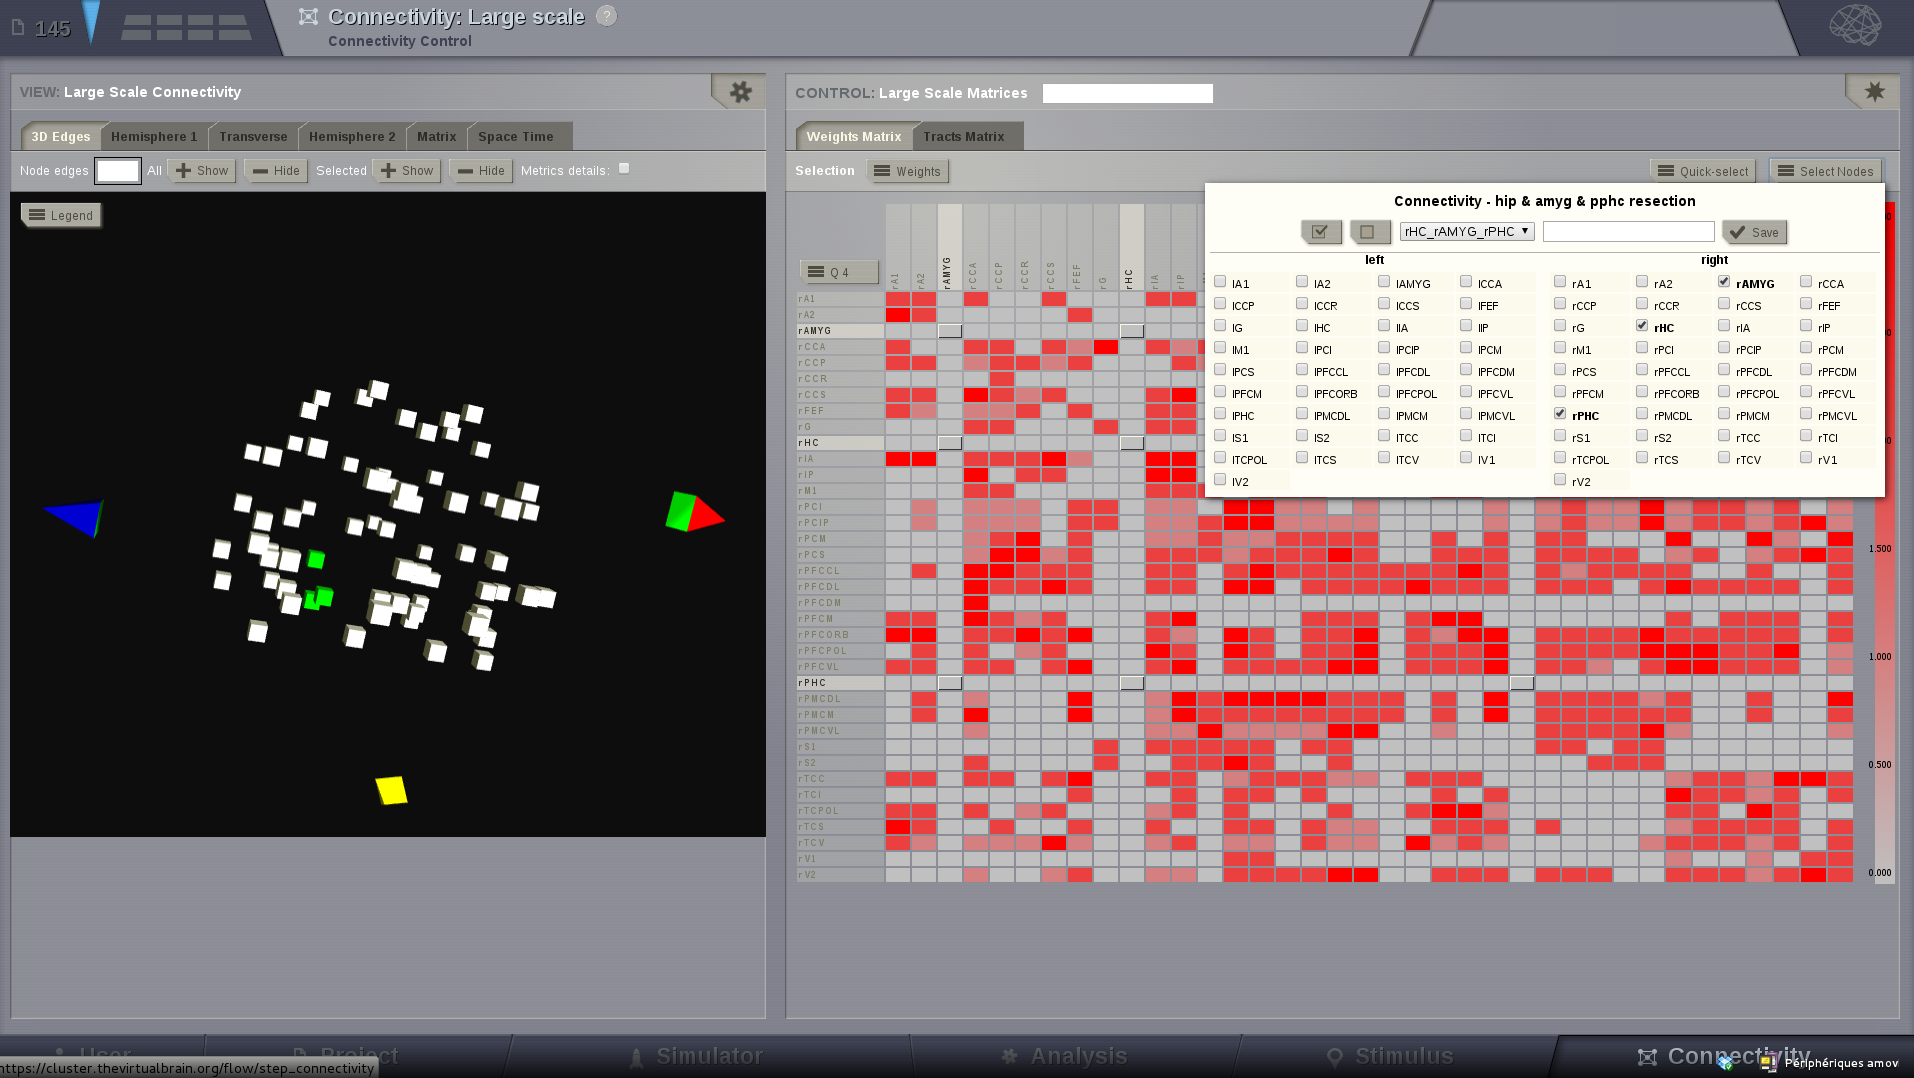
\includegraphics[width=\linewidth]{Handout_UI_ModellingAnEpilepticPatient_ConnectivityMatrixResection}%
  \caption{Focal point for a surface stimulation}%
  \label{fig:resec}%
\end{figure}

\begin{simulation}
  \begin{enumerate}
    \setcounter{enumi}{5}
  \item Click on \underline{Results}, then TimeSeries and visualize the spatial average time series with the a Time Series visualizer.
  Don't forget to increase the \underline{Scaling} and \underline{Select all} channels. (Fig. \ref{fig:ts_resec})
  \end{enumerate}
\end{simulation}

\begin{figure}[h]
  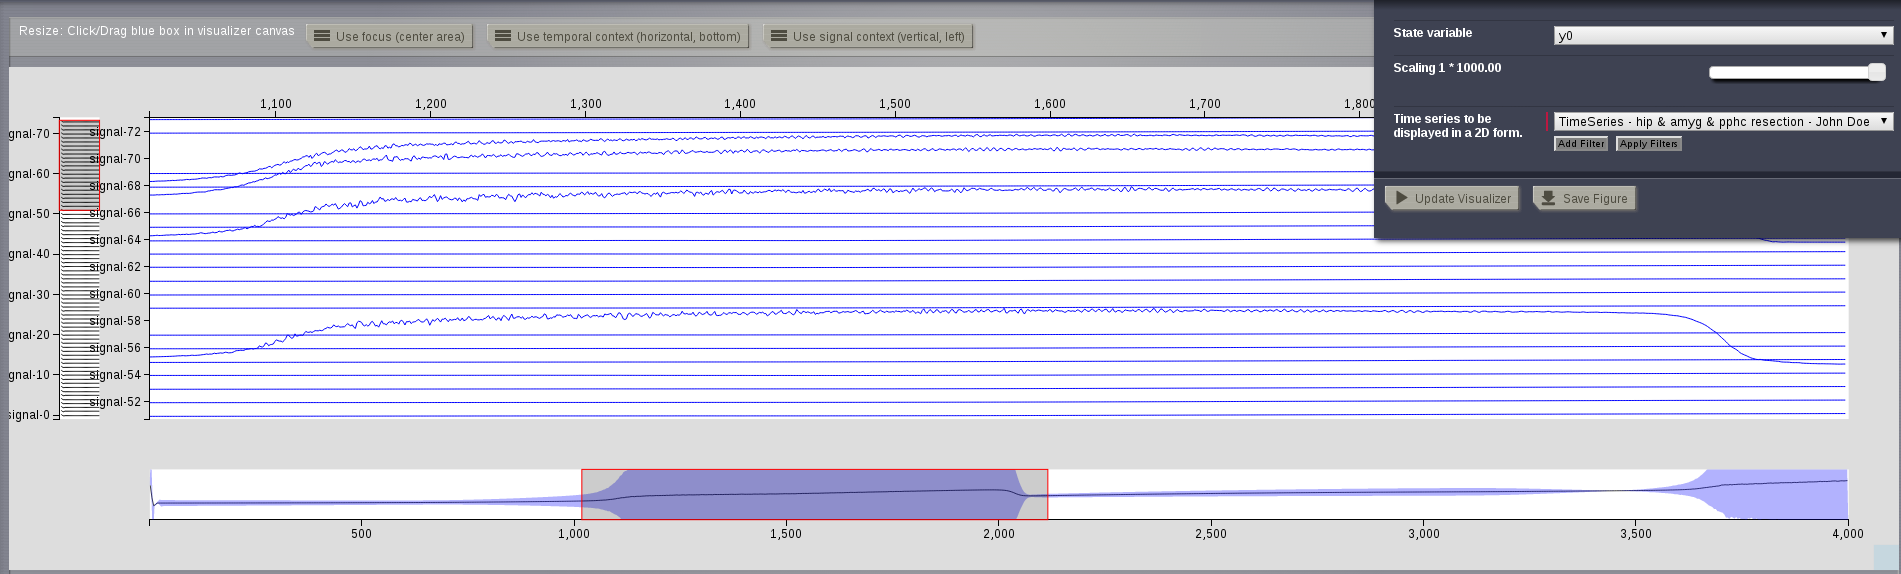
\includegraphics[width=\linewidth]{Handout_UI_ModellingAnEpilepticPatient_TimeSeriesResection}%
  \caption{Time Series after a resection}%
  \label{fig:ts_resec}%
\end{figure}


\section{More Documentation}\label{sec:more-doc}
For more documentation on The Virtual Brain platform, please see the following articles \citep{Sanz-Leon_2013, Woodman_2014}. For more details about the \textbf{Epileptor} model, see  \citep{Jirsa_2014}.


\section{Support}\label{sec:support}

The official TVB webiste is \url{www.thevirtualbrain.org}.  
All the documentation and tutorials are hosted on \url{the-virtual-brain.github.io}.
You'll find our public \smallcaps{git} repository at \url{https://github.com/the-virtual-brain}. For questions and bug reports we have a users group \url{https://groups.google.com/forum/#!forum/tvb-users}

\bibliography{tvb_references}
\bibliographystyle{plainnat}

\end{document}